% ------------------------------------------------------------------------------------------- %
%                                    Resultados e Discussão                                   %
% ------------------------------------------------------------------------------------------- %
\chapter{Resultados}\label{cap:resultados}

Os resultados decorrentes do desenvolvimento deste projeto foram:

\begin{itemize}
	\item Dados resultantes da comparação entre cinco diferentes inteligências e seu desepenho na extração de contextos relevantes presentes em dados de laboratórios e demandas coletados pelo \gls{direc} ao longo dos anos.
	\item A criação de uma aplicação capaz de integrar diferentes modelos de inteligência artificial para a análise linguistica de textos e extração de palavras-chave, bem como a análise de similiaridade entre contextos.
	\item A criação de uma aplicação capaz de mediar a utilização de uma aplicativo mobile com uma aplicação de análise de dados.
	\item Um \gls{mvp} mobile como prova de conceito na utilização das tecnologias empregadas, aceitando a entrada de dados de usuários e oferencendo resultados compreensíveis.
\end{itemize}

% ------------------------------------ Escopo do Sistema ------------------------------------ %
\section{Escopo do sistema}\label{sec:escopoSistema}

O projeto Contrate um Cientista possui dois objetivos principais, sendo eles, a realização de uma análise comparativa entre diferentes modelos de linguagem na terefa de associação de demandas com laboratórios, e a facilitação da formação de parcerias entre o setor produtivo e a expertise científica presente nas universidades através de uma aplicação que, de forma inteligente e automatizada, norteie a tomada de decisões na formação de parcerias. Com estes objetvios postos, é necessaário realizar algumas considerações sobre o escopo do projeto.

O sistema desenvolvido não visa eliminar a necessidade de avaliação das sugestões realizadas pelos profissíonais responsáveis, mas sim fornecer uma ferramenta que auxilie na tomada de decisão, pois nenhum sistema é a prova de falhas. O aplicativo desensolvido é uma prova de conceito e não deve ser visto como uma solução pronta para ambiente de produção, pois mesmo que implemente um mecânismo básico de segurança, não foi desenvolvido com foco na segurança dos dados. Para um cenário de utilização real, a base de dados deve estar presente é um ambiente seguro com acesso controlado, e o armazenamento de dados de usuários deve seguir as regras impostas pela \gls{lgpd}.  

As inteligências \gls{bert}, \gls{gpt}, Azure AI Language e Amazon Comprehend foram escolhidas por se tratar de modelos de linguagem desensolvidos pelas quatro gigantes na área de tecnologia e \gls{ia}, Google, OpenAI, Microsoft e Amazon, respectivamente. A inteligência \gls{yake}, mesmo sendo um modelo análitico, foi escolhido para efeitos de comparação entre \gls{llm} e modelos de análise de texto mais tradicionais. Outro fator que contribuiu para a escolha destas tecnologias foi a disponibilidade de uma \gls{api} de integração e facilidade de implementação.

O sistema abrange dois tipos de usuários, organizações e laboratórios. Ambos os tipos de usuário utilizaram a mesma tela de login para acesso à aplicação, sendo que o conteúdo apresentado após autenticação no sistema difere a depender do tipo de usuário. Organizações são responsáveis pela criação das demandas, cujo conteúdo é analisado contra as informações de todos os laboratórios cadastrados, gerando uma pontuação indicativa de similaridade para cada um. Organizações tambem seram capazes de favoritar os laboratórios de sua preferência por demanda. Laboratórios são responsáveis pelo cadastro de seus recursos relavantes, como descrição do trabalho que efetuam, equipamentos, softwares e certificados, que serão utilizados para a análise e podem ser visualizados pelas organizações.

Para realizar a comparação entre as inteligências integradas foi construído um projeto a parte de teste e benchmarking. Este projeto simula o consumo dos pontos de extremidade expostos pela \gls{api} de aplicação da mesma forma que o aplicativo mobile, porém obtendo informações relevantes para à análise de desempenho, como por exemplo, o tempo de análise de cada inteligência, armazenando as informações obtidas em um banco de dados. Estas informações são utilizadas na conclusão e ajudam a enteder os pontos positivos e possíveis melhorias que podem basear trabalhos futuros.

% ----------------------------------- Modelagem do Sistema ---------------------------------- %
\section{Modelagem do sistema}\label{sec:modelagemSistema}

A maior dificuldade atualmente, se concentra nos responsáveis do departamento que faz esse match entre uma demanda e um cientista nas universidades.
Pensando nisso, o sistema deveria ser de fácil acesso à esses responsáveis, por isso, o App foi uma solução que melhor se enquadraria. 
Finalmente, foi realizado um diagrama para que seja facilmente entendido quais seriam organizados os projetos necessários, juntamente com suas tecnologias, conforme \autoref{fig:fluxograma-comunicacao}.

\begin{figure}[htpb]
    \captionsetup{width=0.43\textwidth}
    \caption{Diagrama da plataforma.}
    \label{fig:fluxograma-comunicacao}
    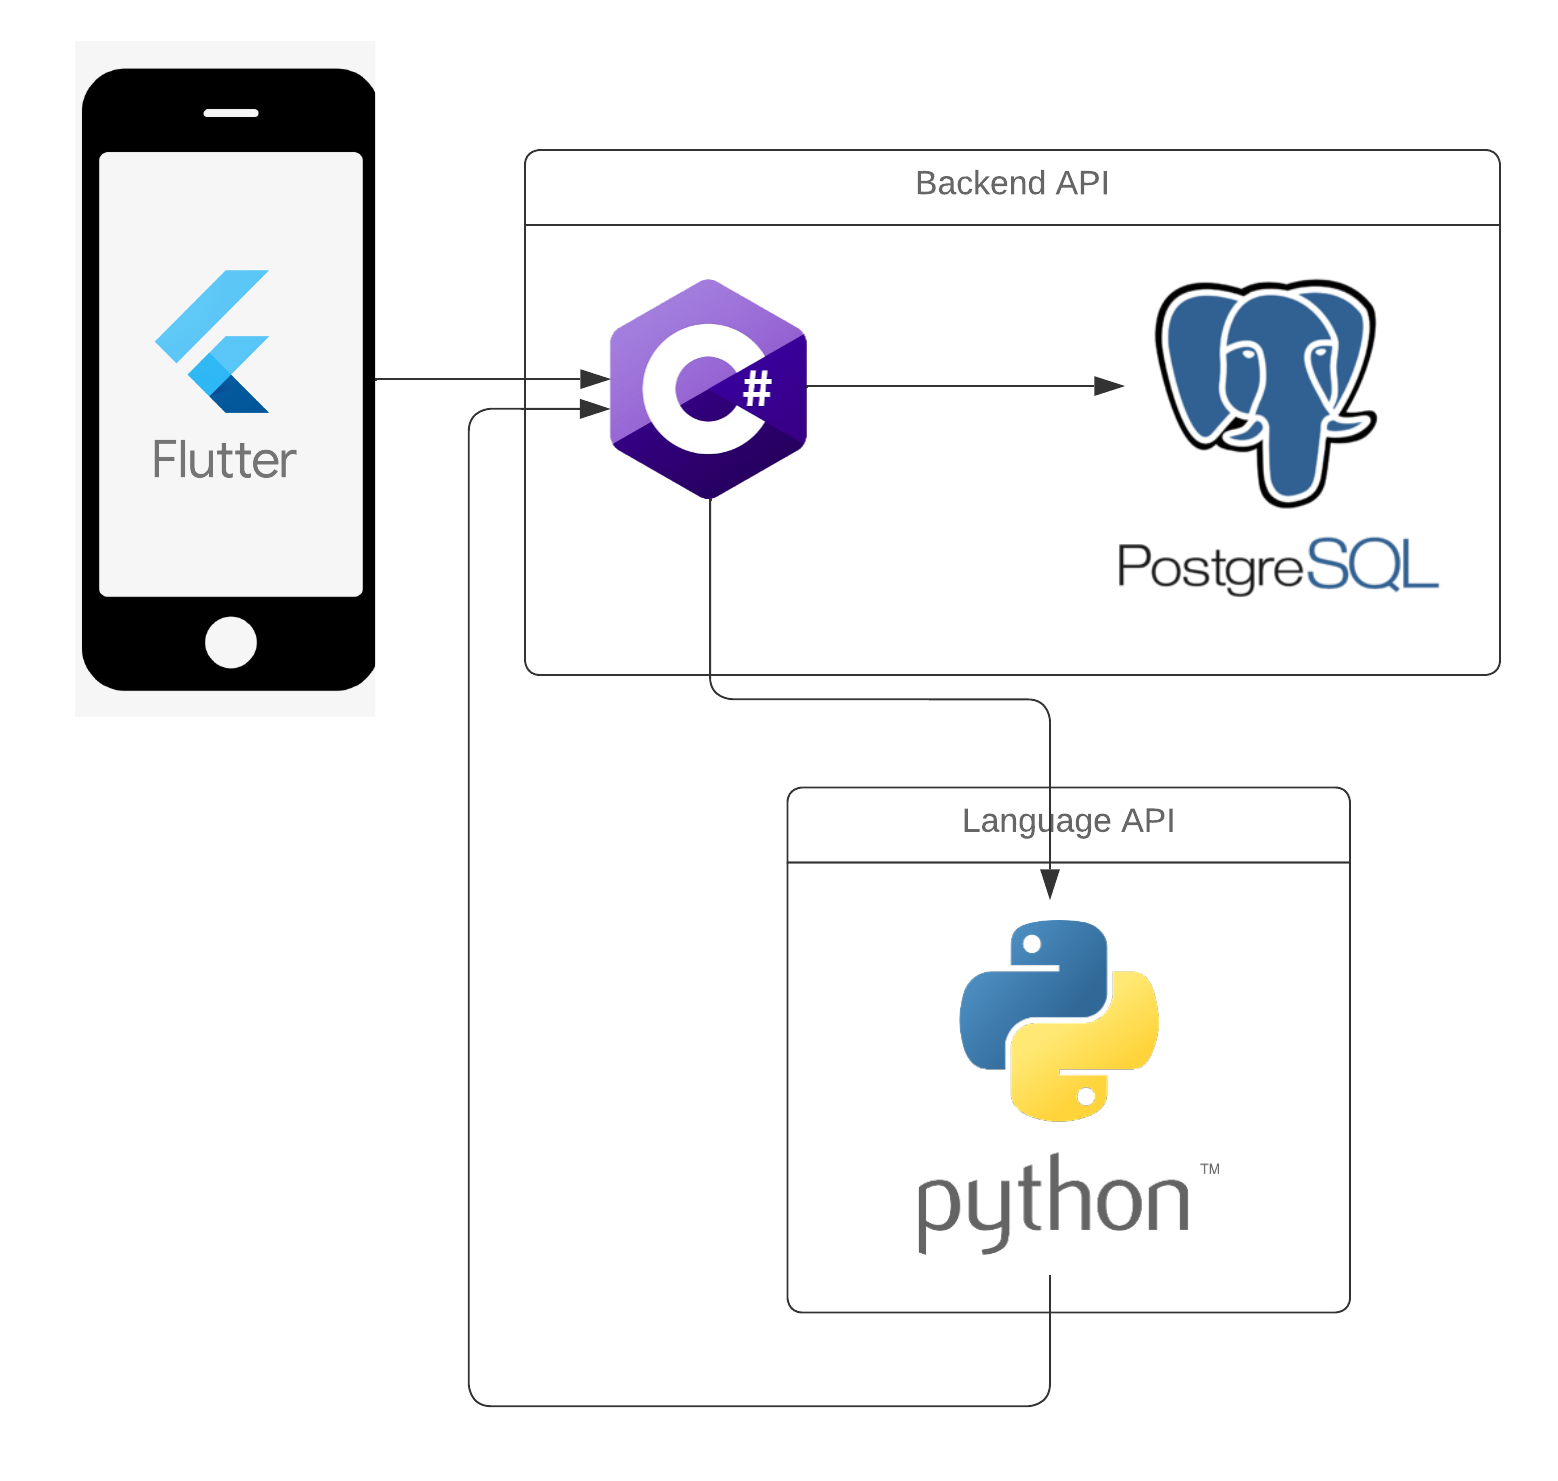
\includegraphics[scale=0.8]{fluxograma-comunicacao}
    \fonte{}
\end{figure}

Como a função principal, é a criação de demandas, foi possível entender melhor os passos através do diagrama \autoref{fig:diagrama-sequencia}.

\begin{figure}[htpb]
    \captionsetup{width=0.43\textwidth}
    \caption{Diagrama de sequência de criação de demanda.}
    \label{fig:diagrama-sequencia}
    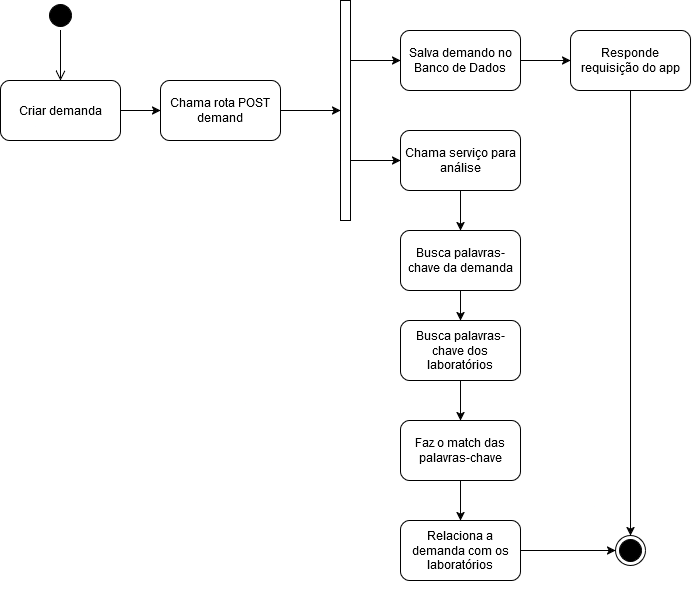
\includegraphics[scale=0.8]{diagrama-sequencia}
    \fonte{}
\end{figure}

\renewcommand{\labelenumii}{\arabic{enumi}.\arabic{enumii}}
\renewcommand{\labelenumiii}{\arabic{enumi}.\arabic{enumii}.\arabic{enumiii}}
\renewcommand{\labelenumiv}{\arabic{enumi}.\arabic{enumii}.\arabic{enumiii}.\arabic{enumiv}}

\subsection{Requisitos Funcionais}\label{subsec:rf}
\begin{enumerate}
    \item O sistema deve disponibilizar um aplicativo
    \item O aplicativo deve ter uma página para o cadastro das organizações
	\begin{enumerate}
		\item Organização deve ter um email para login
		\item Organização deve ter uma senha
		\item Organização deve ter um nome
		\item Organização deve ter um cnpj
		\item Organização deve ter um email para contato
		\item Organização deve permitir uma descrição
	\end{enumerate}
    \item O aplicativo deve ter uma página para o cadastro de laboratórios
	\begin{enumerate}
		\item Laboratório deve ter um email para login
		\item Laboratório deve ter um código
		\item Laboratório deve ter uma data de fundação
		\item Laboratório deve ter palavras-chave
		\item Laboratório deve permitir uma descrição
		\item Laboratório deve permitir o cadastro dos seus certificados
		\item Laboratório deve ter um responsável
		\begin{enumerate}
			\item Responsável deve ter um nome
			\item Responsável deve permitir um departamento
			\item Responsável deve permitir um email
			\item Responsável deve permitir um telefone
		\end{enumerate}
		\item Laboratório deve ter um endereço
		\begin{enumerate}
			\item Endereço deve ter uma rua
			\item Endereço deve ter um número
			\item Endereço deve ter um bairro
			\item Endereço deve ter uma cidade
			\item Endereço deve ter um estado
			\item Endereço deve ter um país
			\item Responsável deve permitir um complemento
		\end{enumerate}
		\item Laboratório deve permitir uma descrição
		\item Laboratório deve permitir uma ou mais redes sociais
		\begin{enumerate}
			\item Rede social deve ter um tipo
			\item Rede social deve ter um link
		\end{enumerate}
		\item Laboratório deve permitir um ou mais equipamentos
		\begin{enumerate}
			\item Equipamento deve ter um nome
			\item Equipamento deve permitir uma descrição
			\item Equipamento deve permitir uma área
		\end{enumerate}
		\item Laboratório deve permitir um ou mais softwares
		\begin{enumerate}
			\item Software deve ter um nome
			\item Software deve permitir uma descrição
			\item Software deve permitir uma área
		\end{enumerate}
	\end{enumerate}
    \item O aplicativo deve ter uma página de login para os usuários
    \item O aplicativo deve permitir que o usuário faça o logout da sua conta
    \item O sistema deve permitir que um usuário visualize e edite as informações do seu perfil no sistema
    \item O aplicativo deve permitir que uma organização crie uma demanda
	\begin{enumerate}
		\item Demanda deve ter um título
		\item Demanda deve ter um departamento
		\item Demanda deve ter benefícios
		\item Demanda deve ter detalhes
		\item Demanda deve ter palavras-chave
		\item Demanda deve permitir uma descrição
		\item Demanda deve permitir restrições
	\end{enumerate}
	\item O sistema deve permitir que uma organização visualize todas suas demandas no sistema
	\item O sistema deve permitir que uma organização favorite laboratórios aptos para uma demanda específica
	\item O sistema deve permitir que uma organização visualize os laboratórios favoritados para cada demanda
	\item O sistema deve permitir que um laboratório visualize as informações da demanda após aquela organização o marcar como favorito
\end{enumerate}

\subsection{Requisitos Não-Funcionais}\label{subsec:rnf}
\begin{enumerate}
\item O sistema deve permitir ser instalado em sistema operacionais Android e iOs
\item O sistema deve ser usado a framework Dart
\item O sistema deve ser servido em C\#
\item O site deverá armazenar dados persistentes com PostgreSQL.
\item O sistema deve armazenar a senha criptografada
\item O sistema deve manter todas as informações protegidas de acordo com permissões do usuário logado
\item O sistema deve mostrar a organização os melhores candidatos para trabalhar naquela demanda
\item O sistema não deve travar até a análise de todos os laboratórios para aquela nova demanda
\end{enumerate}

O diagrama de caso de uso, para fácil visualização dos atores e suas respectivas ações {{diagrama-caso-de-uso}}

O banco de dados foi planejado para comportar os dois tipo de usuários diferentes (laboratório e organização), e para armazenar todos os dados relevantes para análise das demandas, de acordo com o diagrama da \autoref{fig:ERD}.

\begin{figure}[htpb]
    \captionsetup{width=0.43\textwidth}
    \caption{Diagrama de Relação de Entidades do Bando de Dados.}
    \label{fig:ERD}
    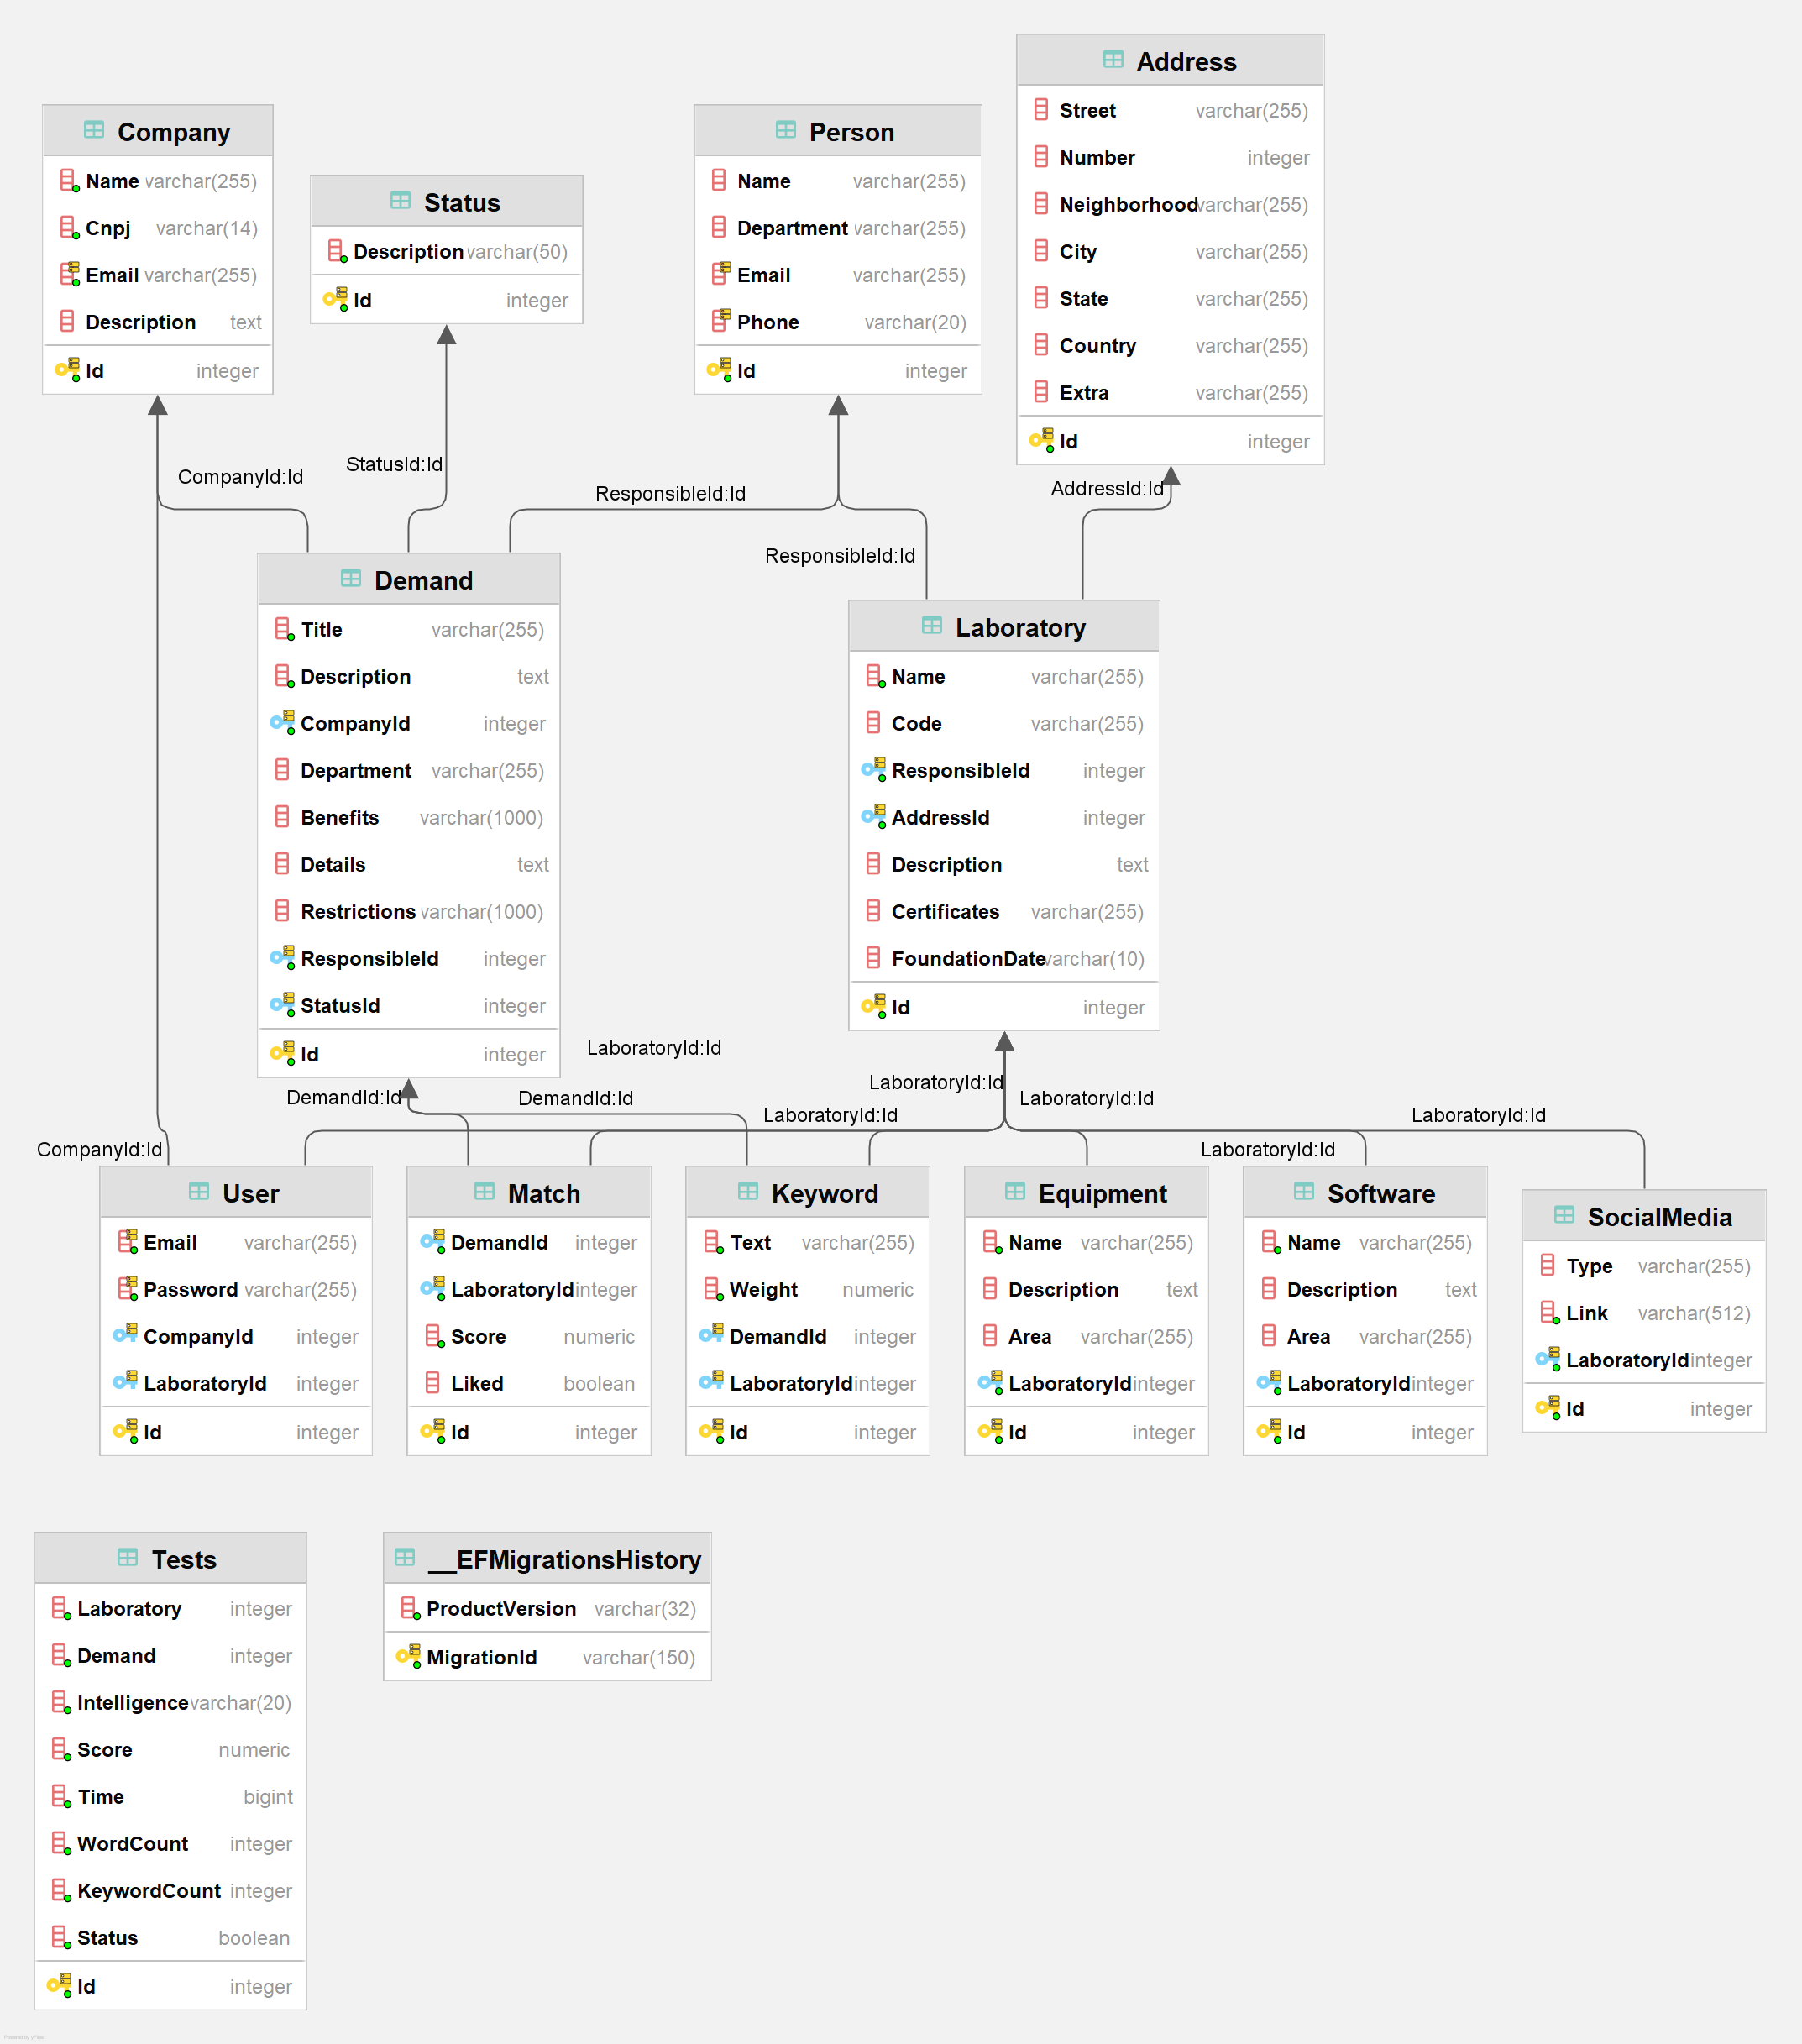
\includegraphics[scale=0.8]{ERD}
    \fonte{}
\end{figure}


% --------------------------------- Apresentação do Sistema --------------------------------- %
\section{Apresentação do sistema}\label{sec:apresentacaoSistema}

O sistema possui uma tela de login inicial, onde o usuário pode preencher seu email e senha, ou fazer um signin. Antes de realizar o signin, o usuário precisa escolher se ele é um laboratório ou organização a se registrar, e então ele é direcionado para seu respectivo formulário para preencher com suas informações.
Após realizar o login e senha, o usuário será redirecionado para sua tela principal, o qual é representado a tela principal da organização na \autoref{fig:pagina-home-org}, onde é mostrada as opções que ele poderá acessar no Aplicativo, como está demonstrado na \autoref{fig:diagrama-navegacao}.

\begin{figure}[htpb]
    \captionsetup{width=0.43\textwidth}
    \caption{Tela inicial de um usuário do tipo organização do aplicativo.}
    \label{fig:pagina-home-org}
    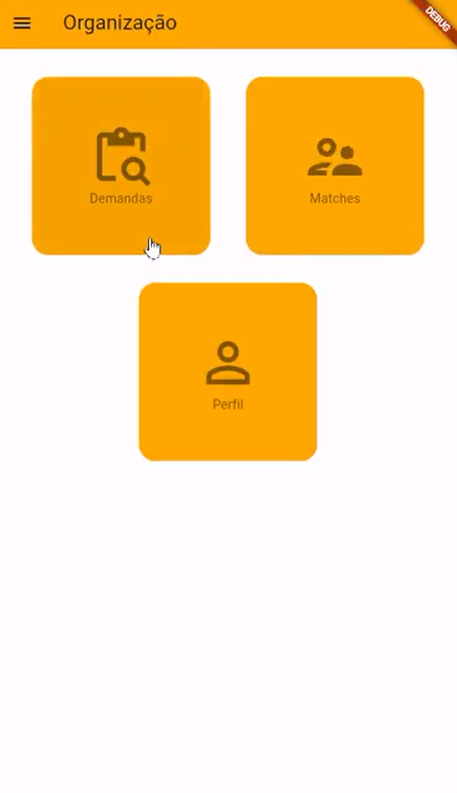
\includegraphics[scale=0.8]{pagina-home-org}
    \fonte{}
\end{figure}

\begin{figure}[htpb]
    \captionsetup{width=0.43\textwidth}
    \caption{Diagrama de navegação ao realizar o login.}
    \label{fig:diagrama-navegacao}
    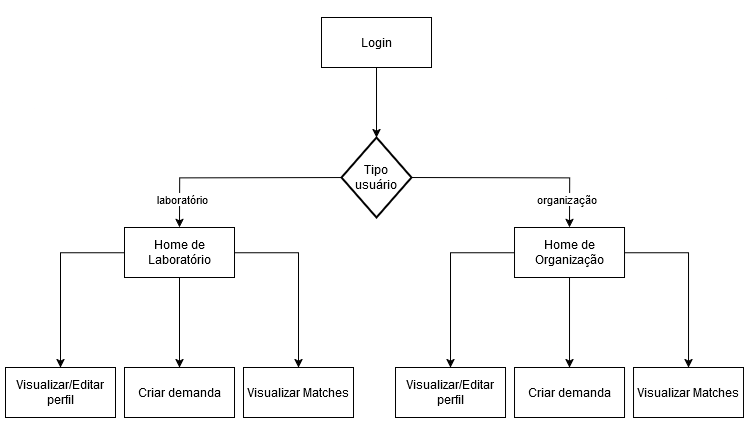
\includegraphics[scale=0.8]{diagrama-navegacao}
    \fonte{}
\end{figure}

Ou seja, uma organização poderá ver seu perfil, as demandas e os matches de todas as demandas, além dos seus detalhes, demonstrado pela \autoref{fig:pagina-matches-detalhes} , enquanto o laboratório poderar ver seu perfil e os matches com os detalhes da demanda do organizador que o marcou como favorito.

\begin{figure}[htpb]
    \captionsetup{width=0.43\textwidth}
    \caption{Tela de detalhes de um match, com o título da demanda, e os detalhes do laboratório, de um usuário do tipo organização do aplicativo.}
    \label{fig:pagina-matches-detalhes}
    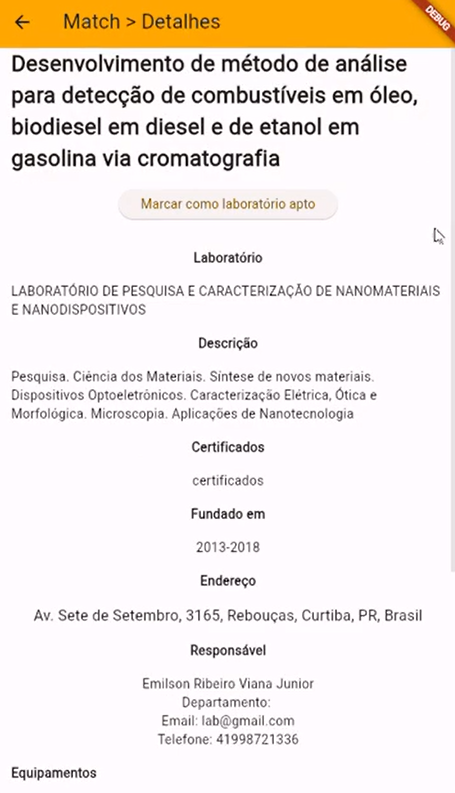
\includegraphics[scale=0.8]{pagina-matches-detalhes}
    \fonte{}
\end{figure}


% --------------------------------- Implementação do Sistema -------------------------------- %
\section{Implementação do sistema}\label{sec:implementacaoSistema}

% Nesta seção é documentada a implementação do sistema com partes relevantes ou exemplos de código, rotinas, funções. Inclui, ainda, a descrição técnica do uso de recursos (componentes, bibliotecas, etc.) da linguagem. Ressalta-se que cada orientador avaliará juntamente com seu orientado o que poderá ser descrito nesta seção. Isso sem que sejam revelados detalhes do sistema que possam comprometer seu uso comercial ou científico ou que a descrição fique muito sucinta ou superficial.

% Em materiais e método estão quais os recursos utilizados, neste capítulo é reportado como esses recursos foram utilizados para resolver o problema.


% Sugere-se colocar listagens curtas de código, enfatizando aspectos específicos das tecnologias utilizadas ou da implementação. Sugere-se, ainda, que o código não seja apresentado sob a forma de print screen, e sim copiado e colado no texto, mantendo, se possível, a formatação. Todas as listagens de código devem ser devidamente explicadas. A explicação deve ser técnica, fundamentada em aspectos conceituais e boas práticas de programação.

% Enfatizar os diferenciais do sistema: procedimentos armazenados, consultas SQL, uso de componentes, uso de padrões de projeto, a forma de uso dos recursos da linguagem. Esses diferenciais são no sentido de explicitar as vantagens, desvantagens, dificuldades e facilidades que esses recursos impetraram no desenvolvimento do sistema em termos técnicos. Esses diferenciais servirão para avaliar pela utilização ou não desses recursos, pelo menos para sistemas iguais ou semelhantes ao reportado no trabalho.

% Reportar a forma como o sistema foi verificado e validado. No sentido de verificar se os requisitos definidos para o mesmo foram atendidos. Os testes podem ser realizados pelo professor orientador, pelos professores que compõem a banca, por pessoas que serviram de base para as informações para o sistema e etc. Os testes podem ser realizados com base em um plano de testes elaborado juntamente com a análise e projeto do sistema. Para validar a implementação podem ser desenvolvidas rotinas de teste unitário.

% Se houver implantação do sistema, mesmo que seja para teste, reportar a forma como isso foi feito, a geração de instaladores, os problemas com ambiente e sistema operacional, incluindo banco de dados e outros. Deixar explícito o procedimento para instalar e usar o sistema.

% Quando for necessário, citar no texto do trabalho nomes de campos, tabelas ou rotinas específicas utilizadas na implementação de um software, utilizar a fonte courier new para destacar esses nomes.

% Um exemplo de listagem de código fonte pode ser observado na \autoref{codigo:classeFoo}, que representa a classe Aluno.

% \begin{sourcecode}[htb]
%     \caption{\label{codigo:classeFoo}Classe Aluno}
%     \begin{lstlisting}[frame=single, language=Java]
% @Entity
% public class Foo {
 
%     @Id
%     @GeneratedValue(strategy = GenerationType.IDENTITY)
%     private Long id;
 
%     private String nome;
    
%     private Integer ra;
     
%     // constructor, getters and setters
% }
% \end{lstlisting}
%     \fonte{}
% \end{sourcecode}